\documentclass[m3380-lec-main.tex]{subfiles}
\setcounter{chapter}{7}

%\DeclareMathOperator{\R}{\mathbb{R}}

\begin{document}


\chapter{Matrix decomposition: $QR$ decomposition}

\section*{Goals}
\begin{enumerate}[1.~]\setlength{\itemsep}{0pt}
\item Discuss least squares regression
\item Discuss the Gram-Schmidt orthonormalization algorithm
\item Discuss $QR$ decomposition using Householder reflectors
\end{enumerate}

\section{Least squares regression} The least squares problem goes back to the beginnings of matrix theory, and in fact to the very problems which Gauss and Legendre considered during the early 1800s. 
Consider the scatter plot in \autoref{fig:scatter}.

\begin{figure}[hbt]
\[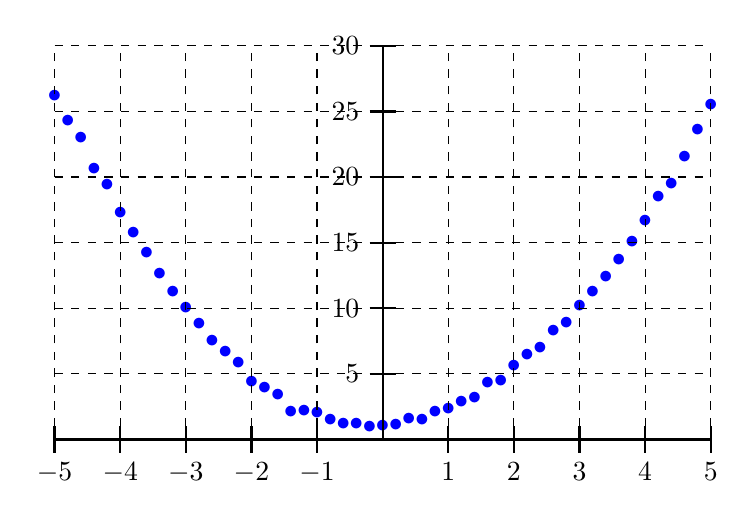
\begin{tikzpicture}[yscale=1/6, xscale=5/6]
\foreach \p in {(-5, 26.18), (-24/5, 24.22), (-23/5, 22.94), (-22/5, 20.55), (-21/5, 19.34), (-4, 17.24), (-19/5, 15.69), (-18/5, 14.17), (-17/5, 12.6), (-16/5, 11.25), (-3, 9.96), (-14/5, 8.78), (-13/5, 7.5), (-12/5, 6.67), (-11/5, 5.78), (-2, 4.34), (-9/5, 3.91), (-8/5, 3.33), (-7/5, 2.09), (-6/5, 2.11), (-1, 1.98), (-4/5, 1.46), (-3/5, 1.18), (-2/5, 1.15), (-1/5, 0.95), (0, 1.0), (1/5, 1.07), (2/5, 1.55), (3/5, 1.43), (4/5, 2.05), (1, 2.3), (6/5, 2.83), (7/5, 3.13), (8/5, 4.31), (9/5, 4.4), (2, 5.59), (11/5, 6.42), (12/5, 6.94), (13/5, 8.23), (14/5, 8.85), (3, 10.13), (16/5, 11.19), (17/5, 12.37), (18/5, 13.64), (19/5, 15.03), (4, 16.64), (21/5, 18.48), (22/5, 19.44), (23/5, 21.53), (24/5, 23.59), (5, 25.49)}{
	\draw \p node {\color{blue}$\bullet$};
};
\draw [thick] (-5,0) -- (5,0)
		(0,0) -- (0,30);
\foreach \x in {-5,-4,-3,-2,-1,1,2,3,4,5}{
	\draw [thick] (\x,-1) node [below] {$\x$} -- (\x,1);
	\draw [dashed] (\x,1) -- (\x,30);
}
\foreach \y in {5,10,15,20,25,30}{
	\draw [thick] (-.2,\y) node [left] {$\y$} -- (.2,\y);
	\draw [dashed] (-5,\y) -- (-.2,\y) (.2,\y) -- (5,\y);
}
\end{tikzpicture}\]
\caption{\label{fig:scatter} A scatter plot.}
\end{figure}
It appears that the points lie along some sort of parabola, but not exactly along the parabola -- there seems to be some error involved in the fit of the curve. A question one might naturally ask is, ``What is the equation of the parabola which best fits the given data?"

This and related questions are most often answered by the process of \emph{least squares regression.} We'll approach this problem by a seemingly unrelated means.

\subsection{Inconsistent systems of equations}
Consider the system \begin{align}\label{eq:incons}\systeme{3x_1-2x_2=4, 2x_1+x_2=9, -3x_1+2x_2=6.}\end{align}
It should be immediately clear that this is an inconsistent system, since not both the first and the third equations can be simultaneously valid. Hence there is no $\vec{x}=\vc{x_1,x_2}$ which satisfies the system. Is it possible then to find some $\bar{x}$ which is the ``best" approximate solution?

We can recast the system \autoref{eq:incons} as a vector and matrix problem (sadly which is still inconsistent) by writing it as $x_1\vec{v}_1+x_2\vec{v}_2 = A\vec{x} = \vec{b}$ where
\begin{align*}
x_1\vec{v_1}+x_2\vec{v_2}   
	&= x_1\begin{bmr}3\\2\\-3\end{bmr} + x_2\begin{bmr}-2\\1\\2\end{bmr}
	= \begin{bmr}3&-2\\2&1\\-3&2\end{bmr} \begin{bmr}x_1\\x_2\end{bmr} 
	=\begin{bmr}4\\9\\6\end{bmr}=\vec{b}.
\end{align*}
What's interesting about this way of writing the system is that now the left-hand side is a \emph{linear combination} of vectors $\vec{v}_1$ and $\vec{v}_2$ and the right-hand side is a vector $\vec{b}$ which \textbf{can not} be written as a linear combination of $\vec{v}_1$ and $\vec{v}_2$.

\begin{defn} A vector $\vec{w}$ is a \emph{linear combination} from a set $S=\set{\vec{v}_1,\vec{v}_2,\ldots,\vec{v}_k}$ if and only if there is a set of scalars $\set{a_1, a_2, \ldots, a_k}$ such that 
\[\vec{w} = a_1\vec{v}_1+a_2\vec{v}_2+\cdots+a_k\vec{v}_k.\] The set of all such vectors $\vec{w}$ is the \emph{span of $S$}. The set $S$ is \emph{linearly independent} if and only if no vector $\vec{v}\in S$ can be written as a linear combination of the vectors in $S\setminus\set{\vec{v}}$.
\end{defn}

So now we can recast our problem in linear algebra terminology: we need to find the vector $\bar{x}\in\lspan\set{\vec{v}_1,\vec{v}_2}$ which is nearest to $\vec{b}$. A convenient fact of working over the real numbers is that we already know how to do this: the shortest path from a line $\ell$ to a point $P$ not on the line is the vector $\vec{r}$ from $X\in\ell$ to $P$ where the line $\overline{XP}$ is perpendicular to $\ell$. To extend this idea to higher dimensions, the vector $\vec{r}$ must be \emph{orthogonal} to any other vector $\vec{v}$ in the linear subspace\footnote{Line, plane, or hyperplane!}.

\begin{defn} Two vectors $\vec{u}, \vec{v}\in\R^n$ are \emph{orthogonal} if and only if $\vec{u}\cdot\vec{v}=0$.
\end{defn}

An easy fact to prove is that the only vector in a space which is orthogonal to every vector in its space is the zero vector.

\begin{thm} Suppose $\vec{u}_0\in\R^n$. If $\vec{u}_0\cdot\vec{v}=0$ for every $\vec{v}\in\R^n$, then $\vec{u}_0 = \vec{0}$.
\end{thm}
\begin{proof} Suppose $\vec{v}\in\R^n$ is an arbitrary vector. Then 
\[\vec{0}\cdot \vec{v} = \sum_{i=1}^n 0v_i = 0,\]
so $\vec{0}$ is orthogonal to every vector in $\R^n$. Now suppose $\vec{u}\neq \vec{0}$; then at least one of the components of $\vec{u}$ is nonzero; suppose that $u_k\neq 0$. Then 
\[\vec{u}\cdot\vec{u} = \sum_{i=0}^n u_i^2 \geq u_k^2 > 0.\]
Hence $\vec{u}$ is not orthogonal to itself, and therefore there is a nonzero vector in $\R^n$ to which $\vec{u}$ is not orthogonal.
\end{proof}

The next theorem establishes that if $\vec{b}\notin\lspan(S)$, then there is some vector in $\lspan(S)$ which is the \emph{closest approximation} of $\vec{b}$ in $\lspan(S)$. As the proof is more complicated, it is omitted.

\begin{thm} Suppose $S=\set{\vec{v}_1,\vec{v}_2,\ldots,\vec{v}_k}$ is a set of linearly independent vectors in $\R^n$ for $n>k$ and $\vec{b}\in\R^n\setminus\lspan(S)$. Then there is a unique vector $\vec{\bar{u}}\in\lspan(S)$ such that the magnitude of $\vec{r}=\vec{b}-\vec{\bar{u}}$ is minimum and $\vec{r}$ is orthogonal to every vector $\vec{u}\in\lspan(S)$.
\end{thm}

Back to our problem, we're looking at vectors $\vec{v}_1 = \vc{3,2,-3}$ and $\vec{v}_2=\vc{-2,1,2}$, and a vector $\vec{b}=\vc{4,9,6}\notin\lspan\set{\vec{v}_1,\vec{v}_2}$. If we let 
\[A = \begin{bmr}3&-2\\2&1\\-3&2\end{bmr},\]
we see that $\vec{u}\in\lspan\set{\vec{v}_1,\vec{v}_2}$ if and only if there is some $\vec{x}=\vc{x_1,x_2}\in\R^2$ such that $A\vec{x}=\vec{u}$. If we want to find $\vec{\bar{u}}=A\vec{\bar{x}}$ such that $\vec{r}=\vec{b}-A\vec{\bar{x}}$ is minimized, it suffices to find $\vec{\bar{x}}$ such that $(A\vec{x})\cdot(\vec{b}-A\vec{\bar{x}})=0$ for all $\vec{x}\in\R^2$.

\begin{lem} If the vectors $\vec{u},\vec{v}\in\R^n$ are considered as $n\times 1$ matrices, then $\vec{u}\cdot\vec{v}=\vec{u}^T\vec{v}$.
\end{lem}

Supposing such a $\vec{\bar{x}}$ exists, 
\begin{align*}
0 = (A\vec{x})\cdot(\vec{b}-A\vec{\bar{x}}) &= (A\vec{x})^T(\vec{b}-A\vec{\bar{x}}) \\
	&= \vec{x}^TA^T(\vec{b}-A\vec{\bar{x}})
\end{align*}
for all $\vec{x}\in\R^2$; but by Theorem 8.3 above, this means that for such a $\vec{\bar{x}}$ to exist it suffices that $A^T\vec{b}-A^TA\vec{\bar{x}}=\vec{0}$, or equivalently that $(A^TA)\vec{\bar{x}} = A^T\vec{b}$. This vector equation has a unique solution exactly when $A^TA$ can be reduced to the identity matrix via Gauss-Jordan elimination. The system of equations corresponding to the equation $(A^TA)\vec{\bar{x}} = A^T\vec{b}$ are called the \emph{normal equations for least squares}.
\begin{thm}[Normal equations for least squares] Suppose $A$ is a $m\times n$ real matrix and $\vec{b}\in\R^m$. The inconsistent system of equations represented by the matrix equation
\[A\vec{x}=\vec{b}\] has a least squares approximation determined by the solution of the normal equations,
\[(A^TA)\vec{\bar{x}}=A^T\vec{b}.\] The residual vector $\vec{r}=\vec{b}-A\vec{\bar{x}}$ is the vector of minimum magnitude in the set \[\set{\vec{b}-A\vec{x}:\vec{x}\in\R^n}.\]
\end{thm}

\section{Application of least squares to curves of best fit} 
The method of least squares applies directly to the originally stated problem of determining a curve of best fit; rather than working an example with a large number of points, let's suppose we have a set of five points through which we desire to find the best-fit parabola\footnote{The curve represented by a polynomial of degree $n$ can be determined uniquely by a set of exactly $n+1$ points; if additional points are specified, the system (in general) becomes overdetermined and inconsistent.}.

\begin{exmp} Suppose we want to best fit a parabola to the points $(-2,1)$, $(-1,2)$, $(0,-2)$, $(1,1)$, and $(3,3)$. If such a parabola were to exist, its quadratic equation $y=a_0+a_1x+a_2x^2$ would need to simultaneously satisfy
\begin{equation}
\systeme{a_0-2a_1+4a_2 = \phantom{-}1,a_0-a_1+a_2 =  \phantom{-}2, a_0=-2, a_0+a_1+a_2= \phantom{-}1, a_0+3a_1+9a_2= \phantom{-}3} 
\quad\Longleftrightarrow\quad A\vec{x} = 
\begin{bmr}
	1 & -2 & 4 \\
	1 & -1 & 1 \\
	1 & 0 & 0 \\
	1 & 1 & 1 \\
	1 & 3 & 9
\end{bmr} \begin{bmr}x_0 \\ x_1 \\ x_2\end{bmr} = \begin{bmr}1 \\ 2 \\ -2 \\ 1 \\ 3\end{bmr} = \vec{b}.
\end{equation}
So we obtain an inconsistent system of equations which can be directly translated to the least squares problem, the solution to which gives the coefficients of the parabola of best fit. We obtain
\begin{align*}
A^TA &= \begin{bmr}5 & 1 & 15 \\
1 & 15 & 19 \\
15 & 19 & 99
\end{bmr} &
A^T\vec{b} &= \begin{bmr}5\\6\\34\end{bmr},
\end{align*}
so augmenting gives
\begin{align*}
\begin{abmr}{3}5 & 1 & 15 & 5 \\
1 & 15 & 19 & 6 \\
15 & 19 & 99 & 34
\end{abmr}&\xto{rref}
\begin{abmr}{3}
1 & 0 & 0 & -\frac{67}{679} \\
0 & 1 & 0 & -\frac{85}{1358} \\
0 & 0 & 1 & \frac{503}{1358}
\end{abmr}.
\end{align*}
Thus the graph of \[y=-\frac{67}{679}-\frac{85}{1358}x+\frac{503}{1358}x^2\] is the best-fit parabola for the five given points.
\end{exmp}

\section{Gram-Schmidt orthonormalization}
A first method for producing an orthogonal matrix from an arbitrary matrix is the Gram-Schmidt algorithm. In essence, the idea is to treat each column of the initial matrix as a vector, and proceed through in order orthogonalizing each vector to those which have previously been orthonormalized.

\begin{exmp} Suppose we begin with two vectors, 
\begin{align*}
\vec{x}_1 &= \vc{1,1,1,1,1}\\
\vec{x}_2 &= \vc{-2,-1,0,1,3},
\end{align*} both in $\R^5$. Then we can imagine somehow in $\R^5$ that these two vectors uniquely determine a plane -- if we let the ``positive horizontal axis" in that plane be determined by the direction of $\vec{x}_1$ and the ``positive vertical axis" by $\vec{x_2}$, we have to determine the projection of $\vec{x}_2$ onto $\vec{x}_1$.
\begin{figure}[hbt]
\[\begin{tikzpicture}
\draw [->] (3,0) -- (6,0) node [right] {$\vec{x}_1$};
\draw [->] (0,0) -- (3,4) node [above right] {$\vec{x}_2$};
\draw [->] (0,0) -- node [below] {$\textrm{proj}_{\vec{x}_1}\vec{x}_2$} (3,0);
\draw [dashed, ->] (0,0) -- node [left] {$\vec{x}_2-\textrm{proj}_{\vec{x}_1}\vec{x}_2$} (0,4);
\draw [dashed] (3,0) -- (3,4);
\end{tikzpicture}\]
\caption{\label{fig:proj2d}Two vectors and the plane they form.}
\end{figure}
Specifically, we want the ``vertical axis" to be in the direction of $\vec{x}_2-\textrm{proj}_{\vec{x}_1}\vec{x}_2$, the component of $\vec{x}_2$ orthogonal to the projection of $\vec{x}_2$ onto $\vec{x}_1$, $\textrm{proj}_{\vec{x}_1}\vec{x}_2$. For an illustration, see \autoref{fig:proj2d}.
\end{exmp}

What is very intuitive about the Gram-Schmidt process is how it extends: to add a third vector $\vec{x}_3$ and orthonormalize it, we subtract from $\vec{x}_3$ its projections onto the two previously-determined ``axes." To add a fourth, we subtract its projection onto each of three previously determined axes. The process continues iterating through the $n$ vectors which form the columns of matrix $X$.

The formula for the projection of a vector $\vec{b}$ onto a vector $\vec{a}$ follows from the correspondence between the dot product and cosine of the interior angle of two vectors: $\vec{a}\cdot\vec{b} = \abs{\vec{a}}\abs{\vec{b}}\cos\alpha$, where $0\leq \alpha\leq \pi$ is the angle between $\vec{a}$ and $\vec{b}$. Thus
\[\proj_{\vec{a}}\vec{b} 
	= \left(\abs{\vec{b}}\cos\alpha\right)\frac{\vec{a}}{\abs{\vec{a}}}
	= \left(\frac{\vec{a}\cdot\vec{b}}{\vec{\abs{a}}}\right)\frac{\vec{a}}{\abs{\vec{a}}}.\]
If it so happens that $\abs{\vec{a}}=1$, then $\vec{a}$ is a \emph{unit vector}, and $\proj_{\vec{a}}\vec{b} = (\vec{a}\cdot\vec{b})\vec{a}$.
\begin{thm}[Gram-Schmidt Orthonormalization] Suppose $S=\set{\vec{x}_1,\vec{x}_2,\cdots,\vec{x}_n}$ is a set of vectors in $\R^m$. Suppose
\begin{align*}
\vec{w}_1 &= \vec{x}_1,\text{ and} \\
\vec{q}_1 &= \vec{w}_1/\abs{\vec{w}_1}.
\end{align*}
Then for each $i=2,3,\ldots,n$, let
\begin{align*}
\vec{w}_i &= \vec{x}_i-\sum_{j=1}^{i-1} (\vec{q}_j\cdot\vec{x}_i)\vec{q}_j,\text{ and}\\
\vec{q}_i &= \vec{w}_i/\abs{\vec{w}_i}.
\end{align*}
Then $Q=\set{\vec{q}_1,\vec{q}_2,\ldots,\vec{q}_n}$ is an orthonormal basis for $\lspan(S)$.
\end{thm}
\begin{proof}
Suppose $1\leq k<\ell\leq n$. Then 
\begin{align*}
\vec{q}_k\cdot\vec{w}_{\ell} &= \vec{q}_k\cdot\vec{x}_{\ell} - \vec{q}_k\cdot\sum_{j=1}^{\ell-1} (\vec{q}_j\cdot\vec{x}_\ell)\vec{q}_j \\
&= \vec{q}_k\cdot\vec{x}_{\ell} - \sum_{j=1}^{\ell-1}(\vec{q}_j\cdot \vec{x}_\ell)(\vec{q}_k\cdot\vec{q}_j)
\end{align*}
Since
\begin{align*}
\vec{q}_k\cdot\vec{q}_j &= \begin{cases} 0&k\neq j\\1&k=j,\end{cases}
\end{align*}
we have $\vec{q}_k\cdot\vec{w}_\ell = \vec{q}_k\cdot\vec{x}_\ell - \vec{q}_k\cdot\vec{x}_\ell = 0$. Thus $\vec{q}_k\cdot\vec{q}_\ell = \frac1{\abs{\vec{w}_\ell}}(\vec{q}_k\cdot\vec{w}_\ell) = 0$ and $\vec{q}_k$ is orthogonal to $\vec{q}_{\ell}$ whenever $k<\ell$. Moreover, 
\[\abs{\vec{q}_k} = \abs{\frac{\vec{w}_k}{\abs{\vec{w}_k}}} = 1,\]
so $Q$ is a set of mutually orthogonal unit vectors. Since $\vec{w}_\ell=\abs{\vec{w}_\ell}\vec{q}_\ell$, each vector $\vec{x}_\ell$ can be written as a linear combination from $\set{\vec{q}_k:k\leq\ell}$; hence any linear combination of vectors in $S$ can be written as a linear combination of vectors in $Q$, and vice versa. Thus $\lspan S=\lspan Q$ and the result holds. 
\end{proof}

The Gram-Schmidt algorithm actually follows directly from the statement of the theorem and the described process, with one minor modification to improve the numerical stability of the algorithm.

\begin{alg}[Modified Gram-Schmidt Orthonormalization] Let \[S=\set{\vec{x}_j:1\leq j\leq n}\] be a set of vectors in $\R^m$. 
\begin{enum}
\item For each $j$ in $\set{1,2,\ldots,n}$, set $\vec{w}_j = \vec{x}_j$. Some of these will be updated later.
\item For $j$ in $\set{1,2,\ldots,n}$, do the following.
\begin{enuma}
\item For each $i<j$, set $\vec{w}_j = \vec{w}_j - (\vec{q_i}\cdot \vec{w}_j)\vec{q}_i$.
\item Let $\vec{q}_j = \frac1{\abs{\vec{w}_j}}\vec{w}_j$.
\end{enuma}
\end{enum}
The set $Q=\set{\vec{q}_j:1\leq j\leq n}$ is an orthonormal basis for $\lspan(S)$.
\end{alg}

\section{$QR$ factorization}
Consider a $m\times n$ matrix $A$; the columns of $A$ can be considered as $n$ vectors in $\R^m$. If those vectors are linearly independent, they span an $n$-dimensional subspace of $\R^m$. The process of Gram-Schmidt orthonormalization performed upon that set of vectors will result in an orthonormal basis for that subspace. Collecting these vectors as the column vectors of a matrix $Q$ gives us the first half of the $QR$ factorization of $A$. The matrix $R$ is produced as an upper-triangular matrix recording the magnitudes of the projections removed in each iteration of step 2a above, along with the scaling factors of step 2b. That is, $R=[r_{i,j}]$ is a $n\times n$ matrix with
\begin{align}\label{eq:rmatrix}
r_{i,j} &= \begin{cases}
	\vec{q}_i\cdot \vec{w}_j, & i<j \\
	\abs{\vec{w}_j}, & i=j \\
	0, &i>j.
	\end{cases}
\end{align}
This means that the order in which elements of $R$ are recorded during the algorithm will be sort of ``transpose'' to the normal order: $r_{1,1}$, $r_{1,2}$, $r_{2,2}$, $r_{1,3}$, $r_{2,3}$, $r_{3,3}$, and so on. 

The matrices $Q$ and $R$ produced as just described are the \emph{reduced $QR$ factorization of $A$}. If it exists, it is customary to add $m-n$ extra columns to $A$; these can be any column vectors linearly independent from the original columns of $A$, so it is often the case that the columns added correspond to vectors $\vc{1,0,0,\ldots}$, $\vc{0,1,0,\ldots}$, $\vc{0,0,1,\ldots}$, and so on. The orthonormal basis will then be a full basis for $\R^m$ containing $m$ vectors; in order that $A=QR$, it must be that $R$ is a $m\times n$ matrix. In fact this is the case, with $R=[r_{i,j}]$ the $m\times n$ matrix with the same formula from \autoref{eq:rmatrix} determining its elements. This different factorization is called the \emph{full $QR$ factorization of $A$}.

\begin{defn} A square matrix $Q$ is \emph{orthogonal} if and only if $Q^T=Q^{-1}$.
\end{defn}

\begin{thm} Suppose $QR=A$ is the full $QR$ factorization of $A$. Then $Q$ is an orthogonal matrix.
\end{thm}
\begin{proof}
Consider $Q^TQ = [m_{i,j}]$. Then 
\[m_{i,j} = \vec{q}_i\cdot\vec{q}_j = \begin{cases}0&i\neq j\\1&i=j,\end{cases}\] and the desired result holds.
\end{proof}

\subsection{Utility of $QR$ factorization}
While we can use the $QR$ factorization to solve a system of equations, it is approximately three times more complicated than $LU$ decomposition. However, $QR$ decomposition can avoid a problem called \emph{ill-conditioning} in solving the least squares problem.

\begin{alg}[Least squares by $QR$ factorization]
Given the $m\times n$ inconsistent system of equations represented by $A\vec{x}=\vec{b}$, let $QR=A$ be the full $QR$ factorization of $A$ and let
\begin{align*}
\hat{R} &= \text{upper $n\times n$ submatrix of $R$} \\
\hat{\vec{d}} &= \text{upper $n$ entries of }\vec{d}=Q^T\vec{b}
\end{align*}
Then the solution to $\hat{R}\vec{\bar{x}}=\hat{\vec{d}}$ is the least squares solution $\bar{\vec{x}}$.
\end{alg}

\section{$QR$ factorization by Householder reflectors}

Another algorithm for determining the $QR$ factorization of a matrix which requires fewer operations and is less susceptible to rounding error is the method of Householder reflectors. The method depends upon the following theorem.
\begin{rem} Throughout this section, it will be important to remember that if $\vec{x}_1,\vec{x}_2\in\R^n$, then $\vec{x}_1^T\vec{x}_2 = \vec{x}_1\cdot\vec{x}_2$. The transpose notation makes certain calculations and formulas nicer, or easier to prove.
\end{rem}

\begin{thm} Suppose $\vec{x},\vec{w}\in\R^n$ have $\abs{\vec{x}}=\abs{\vec{w}}$. Then $\vec{w}-\vec{x}$ and $\vec{w}+\vec{x}$ are orthogonal.
\end{thm}
\begin{proof} The proof is made visually in \autoref{fig:refl_thm1}, but is nonetheless simple to show algebraically:
\[ (\vec{w}-\vec{x})^T(\vec{w}+\vec{x}) = \vec{w}^T\vec{w}-\vec{x}^T\vec{w}+\vec{w}^T\vec{x}-\vec{x}^T\vec{x} = \abs{\vec{w}}^2-\abs{\vec{x}}^2 = 0. \]
Geometrically, the result follows as the vectors $\vec{x}$ and $\vec{w}$ form two legs of an isosceles triangle, $\vec{w}-\vec{x}$ the base, and $\vec{w}+\vec{x}$ the angle bisector of the angle subtended by the legs.
\end{proof}

\begin{figure}[hbt]
\[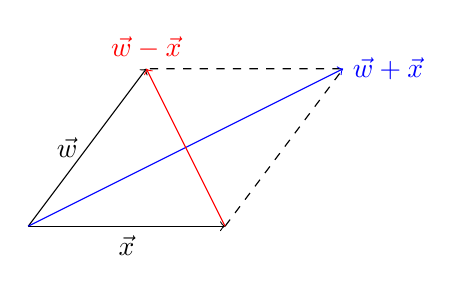
\begin{tikzpicture}[scale=1/2]
\draw [->] (0,0) -- node [left] {$\vec{w}$} (3,4);
\draw [->] (0,0) -- node [below] {$\vec{x}$} (5,0);
\draw [dashed] (5,0) -- (8,4) -- (3,4);
\draw [->, draw = blue]  (0,0) -- (8,4) node [right] {\color{blue}$\vec{w}+\vec{x}$} ;
\draw [->, draw = red] (5,0) -- (3,4) node [above] {\color{red}$\vec{w}-\vec{x}$} ;
\end{tikzpicture}\]
\caption{\label{fig:refl_thm1} Orthogonality of $\vec{w}-\vec{x}$ and $\vec{w}+\vec{x}$ in $\R^n$.}
\end{figure}

Give two such vectors $\vec{x},\vec{w}\in\R^n$, define $\vec{v}=\vec{w}-\vec{x}$, and consider the matrix
\[P = \frac{\vec{v}\vec{v}^T}{\vec{v}^T\vec{v}}.\]
While it may be confusing to think that this is a matrix, recall: since $\vec{v}$ is an $n\times 1$ column matrix, $\vec{v}\vec{v}^T$ is an $n\times n$ symmetric matrix. In fact, 
\begin{align*} P^2 &= \frac{\vec{v}\vec{v}^T}{\vec{v}^T\vec{v}}\frac{\vec{v}\vec{v}^T}{\vec{v}^T\vec{v}} = \frac{\vec{v}(\vec{v}^T\vec{v})\vec{v}^T}{(\vec{v}^T\vec{v})^2} = \frac{\vec{v}\vec{v}^T}{\vec{v}^T\vec{v}} = P,
\text{ and} 
&
P\vec{v} &= \frac{\vec{v}\vec{v}^T}{\vec{v}^T\vec{v}}\vec{v} = \frac{\vec{v}(\vec{v}^T\vec{v})}{\vec{v}^T\vec{v}} = \vec{v}.
\end{align*}
A matrix satisfying $P^2=P$ is called a \emph{projection matrix.} The purpose of using $P$ is that $\vec{x}-P\vec{x}$ is the projection of $\vec{x}$ onto $\vec{y+x}$, and therefore $\vec{x}-2P\vec{x} = \vec{w}$!

\begin{thm} Let $\vec{x},\vec{w}\in\R^n$ with $\abs{\vec{x}}=\abs{\vec{w}}$, and suppose $\vec{v} = \vec{w}-\vec{x}$. Then the matrix
\[ H = I-2\frac{\vec{v}\vec{v}^T}{\vec{v}^T\vec{v}} \]
is a \emph{Householder reflector}, and is a symmetric orthogonal matrix with $H\vec{x}=\vec{w}$.
\end{thm} 

For brevity, I'll refer to the $QR$ factorization by Householder reflectors as HHQR. The process of HHQR for a matrix $A$ iterates through the columns of $A$ just like Gram-Schmidt, but with far less numerical instability. We'll explain the process without use of an example, as the process becomes extremely unwieldy in exact arithmetic.

Suppose we begin with a $m\times n$ matrix\footnote{The discussion of the method contained here originally appears in Timothy Sauer's excellent \emph{Numerical Analysis, 2nd edition}.} $A = [a_{i,j}]$, where $m>n$. We will choose as our first vector $\vec{x}_1 = \vc{a_{1,1},a_{2,1},\ldots, a_{m,1}}$, the first column of $A$. Since we desire to reflect it onto a coordinate axis vector of the same magnitude, we can choose $\vec{w_1}=\vc{\pm\abs{\vec{x}_1},0,0,\ldots,0}$. Since subtracting nearly identical floating point numbers is problematic and leads to rounding error, we will choose the sign of the first coordinate of $\vec{w}_1$ to be the opposite of the sign of the first coordinate of $\vec{x}_1$. This allows us to determine the first Householder reflector $H_1$ such that $H_1\vec{x}_1 = \vec{w}_1$. Now, putting $R_1 = H_1A$ gives us a matrix whose first column is $\vec{w}_1$, by construction; notably, this is the first iteration and in the first column $R_1$ is the start of an upper triangular matrix. Specifically, if we write $R_1=[r_{i,j}]$, we have $r_{i,1} = 0$ whenever $i>1$.

In order to continue this process, we will produce from $R_1$ a new matrix $R_2=[r_{i,j}]$ which has $r_{i,j}=0$  whenever $i>j$ and $j\leq 2$. We do so by ignoring the first row and column of $R_1$; doing so gives us $R'_1$, an $(m-1)\times(n-1)$ matrix. If we let $\vec{x}_2$ be the first column of $R'_1$ and $\vec{w}_2=\vc{\pm\abs{\vec{x}_2},0,0,\ldots,0}$, we can find the Householder reflector $\hat{H}_2$ such that $\hat{H}_2\vec{x}_2=\vec{w}_2$. Say then that $\hat{H}_2 = [\hat{h}_{i,j}]$. We will create our ``real" reflection matrix by inserting $\hat{H}_2$ into the bottom right corner of an identity matrix. Here is the formula for $h_{i,j}$ along with the more intuitive picture diagram:
\[h_{i,j} = \begin{cases}
1, & i<2\text{ or }j<2,\text{ and }i=j \\
0, & i<2\text{ or }j<2,\text{ and }i\neq j \\
\hat{h}_{i,j}, & i,j\geq 2
\end{cases},\qquad\text{or}\qquad
H_2 = \begin{augbmc}{1}{3}
1 & 0 & \cdots & 0 \\ \hline
0 &   &   &   \\
\vdots &   & \hat{H}_2 &   \\
0 &   &   &   
\end{augbmc}.\]
Then $R_2=H_2R_1=H_2H_1A$.

We continue this process in the way established: at each step, we reflect the first column of a submatrix onto a coordinate-axis vector of the same length, flipping signs of the first coordinate, and after processing $n$ columns in this way we have $R=H_nH_{n-1}\cdots H_2H_1A$, which is an upper triangular matrix. Moreover, the matrices $H_j$ are all orthogonal matrices, so $H_j^{-1}=H_j$. Hence we obtain
\[QR = (H_1H_2\cdots H_{n-1}H_n) R = A.\]

\begin{alg}[HHQR]
Suppose $A$ is a $m\times n$ matrix.
\begin{enum}
\item Let $Q$ be the $m\times m$ identity matrix.
\item Let $R$ be a floating point copy of $A$.
\item In the $j^\text{th}$ column, for $j=1,2,\ldots,n$:
\begin{enuma}
\item Let $\vec{x}=\vc{r_{j,j},r_{j+1,j},\ldots,r_{m,j}}$
\item Let $\vec{w}=\vc{\pm\abs{\vec{x}},0,0,\ldots,0}$ with the first coordinate having the opposite sign as in $\vec{x}$.
\item Let $\vec{v}=\vec{w}-\vec{x}$ and $\hat{H}=I-2\frac{\vec{v}\vec{v}^T}{\vec{v}^T\vec{v}}$.
\item Let $H$ be the $m\times m$ identity matrix with $\hat{H}$ replacing its bottom right corner.
\item Set $Q=QH$
\item Set $R=HR$
\end{enuma}\end{enum}
When the algorithm terminates, $QR=A$.
\end{alg}

Here's Python code which implements HHQR when $A$ is specified as a list of lists rather than a matrix. Notice how local functions \verb|sign|, \verb|householder|, and \verb|times| are defined within the \verb|hhqr| function.

\smallskip{\fn\begin{verbatim}
from math import sqrt

def hhqr(A):
    sign = lambda x: 1 if x>0 else (-1 if x<0 else 0)
    
    def householder(xvec,wvec):
        vvec = [wvec[i]-x for i,x in enumerate(xvec)]
        d = sum([v**2 for v in vvec])
        H = [[(1 if i==j else 0) - 2*vvec[i]*vvec[j]/d for
              j in range(len(vvec))] for i in range(len(vvec))]
        return H
    
    def times(A,B):
        return [[sum([A[i][k]*B[k][j] for k in range(len(A[0]))]) for
                 j in range(len(B[0]))] for i in range(len(A))]
    
    m = len(A)
    n = len(A[0])
    Q = [[(1 if i==j else 0) for j in range(m)] for i in range(m)]
    R = [[float(x) for x in row] for row in A]
    for j in range(n):
        x = [R[i][j] for i in range(j,m)]
        w = [-sign(x[0])*sqrt(sum([xi**2 for xi in x]))]+(m-j-1)*[0]
        hh = householder(x,w)
        H = [[(1 if k==l else 0) if (k<j or l<j) else hh[k-j][l-j] for
              l in range(m)] for k in range(m)]
        Q = times(Q,H)
        R = times(H,R)
    ##########################################################################
    ## Everything after this is just to print the verification output nicely.
    print('Verification: Q*R-A\n')
    mat = times(Q,R)
    mat = [[mat[i][j] - A[i][j] for j in range(n)] for i in range(m)]
    clens = [max([len(str(mat[i][j])) for i in range(m)]) for j in range(n)]
    out = ''
    for i in range(m):
        out += '[ '
        for j in range(n):
            l = len(str(mat[i][j]))
            out += (clens[j]-l)*' '+str(mat[i][j])+', '
        out = out[:-2] + ' ]\n'
    print(out)
    ##########################################################################
    ## Except this, of course.
    return Q,R
\end{verbatim}
}\smallskip\noindent



%\begin{exmp} Suppose we want to find the HHQR of
%\[A = \begin{bmr}
%1 & -4 & 5 \\
%2 & 3 & 5 \\
%2 & 2 & -4 \\
%4 & 6 & 0
%\end{bmr}\]
%We'll start by taking $\vec{x}=\vc{1,2,2,4}$, the first column of $A$, and reflect it onto a vector of the same magnitude in a coordinate direction. To make this easy, we'll reflect it onto $\vec{w} = \vc{-\abs{\vec{x}},0,0,0}=\vc{-5,0,0,0}$. We've chosen to make the first coordinate negative because it is the opposite sign as the first coordinate of $\vec{x}$, which will (in the general algorithm) help us avoid subtracting two numbers which are very close to equal. Then the vector $\vec{v}=\vec{w}-\vec{x} = \vc{6,2,2,4}$ has $\vec{v}^T\vec{v} = 60$, and
%\begin{align*}
%\frac{\vec{v}\vec{v}^T}{\vec{v}^T\vec{v}} = \frac1{60}
%\begin{bmr}
%36 & 12 & 12 & 24 \\
%12 & 4 & 4 & 8 \\
%12 & 4 & 4 & 8 \\
%24 & 8 & 8 & 16
%\end{bmr} = \begin{bmr}
%\frac{3}{5} & \frac{1}{5} & \frac{1}{5} & \frac{2}{5} \\
%\frac{1}{5} & \frac{1}{15} & \frac{1}{15} & \frac{2}{15} \\
%\frac{1}{5} & \frac{1}{15} & \frac{1}{15} & \frac{2}{15} \\
%\frac{2}{5} & \frac{2}{15} & \frac{2}{15} & \frac{4}{15}
%\end{bmr} = P_1
%\end{align*}
%is our first projection matrix. Creating the Householder reflector for this projection gives us
%\[ H_1 = I-2P_1 = \begin{bmr}
%-\frac{1}{5} & -\frac{2}{5} & -\frac{2}{5} & -\frac{4}{5} \\
%-\frac{2}{5} & \frac{13}{15} & -\frac{2}{15} & -\frac{4}{15} \\
%-\frac{2}{5} & -\frac{2}{15} & \frac{13}{15} & -\frac{4}{15} \\
%-\frac{4}{5} & -\frac{4}{15} & -\frac{4}{15} & \frac{7}{15}
%\end{bmr}\qquad\text{and}\qquad
% R_1 = H_1A = \begin{augbmr}{1}{2}
%-5 & -6 & -\frac{7}{5} \\ \hline
%0 & \frac{7}{3} & \frac{43}{15} \\
%0 & \frac{4}{3} & -\frac{92}{15} \\
%0 & \frac{14}{3} & -\frac{64}{15}
%\end{augbmr}.\]
%We've now completed our first step -- we've mapped the first column of $A$ onto a vector of the same magnitude but along a coordinate axis. The matrix on the right is subdivided into four regions to highlight a crucial fact in the HHQR process: we can treat the submatrix on the lower right as what we want to factorize, and if we continue to move down through submatrices in this manner should produce a sequence $R_1,R_2,\ldots,R_k$ where $R_k$ is an upper triangular matrix (though not a square upper triangular matrix).
%
%To that purpose let's now set 
%\begin{align*}
%\vec{x} &= \vc{\frac73,\frac43,\frac{14}3}, \\
%\vec{w} &= \vc{-\sqrt{29},0,0}.
%\end{align*}
%Then following the process, we get $\vec{v}=\vec{w}-\vec{x} = \vc{-\frac{7+3\sqrt{29}}3,-\frac43,-\frac{14}3}$. The numbers here begin to become unwieldy in exact arithmetic, but we can persevere. We obtain 
%\[\vec{v}^T\vec{v} = \frac{14\sqrt{29}+174}3,\]
%which in turn gives 
%\begin{align*}
%P_2 = \frac{\vec{v}\vec{v}^T}{\vec{v}^T\vec{v}} &= \frac3{14\sqrt{29}+174}
%\begin{bmr}
%\frac19\left(3\sqrt{29}+7\right)^2 & \frac43\sqrt{29}+\frac{28}9 & \frac{14}3\sqrt{29}+\frac{98}9 \\
%\frac43\sqrt{29}+\frac{28}9 & \frac{16}9 & \frac{56}9 \\
%\frac{14}3\sqrt{29}+\frac{98}9 & \frac{56}9 & \frac{196}9
%\end{bmr} \\
%&= \begin{bmr}
%\frac{{\left(3  \sqrt{29} + 7\right)}^{2}}{{\left(3  \sqrt{29} + 7\right)}^{2} + 212} & \frac{4  {\left(3  \sqrt{29} + 7\right)}}{{\left(3  \sqrt{29} + 7\right)}^{2} + 212} & \frac{14  {\left(3  \sqrt{29} + 7\right)}}{{\left(3  \sqrt{29} + 7\right)}^{2} + 212} \\
%\frac{4  {\left(3  \sqrt{29} + 7\right)}}{{\left(3  \sqrt{29} + 7\right)}^{2} + 212} & \frac{16}{{\left(3  \sqrt{29} + 7\right)}^{2} + 212} & \frac{56}{{\left(3  \sqrt{29} + 7\right)}^{2} + 212} \\
%\frac{14  {\left(3  \sqrt{29} + 7\right)}}{{\left(3  \sqrt{29} + 7\right)}^{2} + 212} & \frac{56}{{\left(3  \sqrt{29} + 7\right)}^{2} + 212} & \frac{196}{{\left(3  \sqrt{29} + 7\right)}^{2} + 212}
%\end{bmr}.
%\end{align*}
%This is a fairly unappealing matrix, but not uncommonly so for this process. We continue with 
%\[ \hat{H}_2 = I-2P_2 = \begin{bmr}
%1-\frac{{2\left(3  \sqrt{29} + 7\right)}^{2}}{{\left(3  \sqrt{29} + 7\right)}^{2} + 212} 
%	& -\frac{8  {\left(3  \sqrt{29} + 7\right)}}{{\left(3  \sqrt{29} + 7\right)}^{2} + 212} 
%	& -\frac{28  {\left(3  \sqrt{29} + 7\right)}}{{\left(3  \sqrt{29} + 7\right)}^{2} + 212} \\
%-\frac{8  {\left(3  \sqrt{29} + 7\right)}}{{\left(3  \sqrt{29} + 7\right)}^{2} + 212} 
%	& 1-\frac{32}{{\left(3  \sqrt{29} + 7\right)}^{2} + 212} 
%	& \frac{56}{{\left(3  \sqrt{29} + 7\right)}^{2} + 212} \\
%-\frac{28  {\left(3  \sqrt{29} + 7\right)}}{{\left(3  \sqrt{29} + 7\right)}^{2} + 212} 
%	& -\frac{112}{{\left(3  \sqrt{29} + 7\right)}^{2} + 212} 
%	& 1-\frac{392}{{\left(3  \sqrt{29} + 7\right)}^{2} + 212}
%\end{bmr}\]
%To build our matrix $H_2$ from $\hat{H}_2$, we will insert $\hat{H}_2$ into the lower-right corner of an identity matrix\footnote{Technically, we're defining $H_2 = [h_{i,j}]$ where \[h_{i,j} = \begin{cases}
%\begin{cases} 1, & i=j \\ 0, &i\neq j\end{cases}, &i<2\text{ or }j<2 \\ \hat{H}_2(i,j), & \text{otherwise}\end{cases}.\] That's very cumbersome.} which results in 
%\[ H_2 = \begin{augbmc}{1}{3} 1 & 0 & 0 & 0 \\ \hline 0 & & & \\ 0 & & \hat{H}_2 & \\ 0 & & & \end{augbmc}.\]
%\end{exmp}
\end{document}